%%
%% This is file `sample-sigconf.tex',
%% generated with the docstrip utility.
%%
%% The original source files were:
%%
%% samples.dtx  (with options: `sigconf')
%% 
%% IMPORTANT NOTICE:
%% 
%% For the copyright see the source file.
%% 
%% Any modified versions of this file must be renamed
%% with new filenames distinct from sample-sigconf.tex.
%% 
%% For distribution of the original source see the terms
%% for copying and modification in the file samples.dtx.
%% 
%% This generated file may be distributed as long as the
%% original source files, as listed above, are part of the
%% same distribution. (The sources need not necessarily be
%% in the same archive or directory.)
%%
%%
%% Commands for TeXCount
%TC:macro \cite [option:text,text]
%TC:macro \citep [option:text,text]
%TC:macro \citet [option:text,text]
%TC:envir table 0 1
%TC:envir table* 0 1
%TC:envir tabular [ignore] word
%TC:envir displaymath 0 word
%TC:envir math 0 word
%TC:envir comment 0 0
%%
%%
%% The first command in your LaTeX source must be the \documentclass command.
\documentclass[sigconf]{acmart}
\usepackage[UTF8, heading=false, scheme=plain]{ctex}
\usepackage[linesnumbered,ruled]{algorithm2e}


%%
%% \BibTeX command to typeset BibTeX logo in the docs
\AtBeginDocument{%
  \providecommand\BibTeX{{%
    \normalfont B\kern-0.5em{\scshape i\kern-0.25em b}\kern-0.8em\TeX}}}

%% Rights management information.  This information is sent to you
%% when you complete the rights form.  These commands have SAMPLE
%% values in them; it is your responsibility as an author to replace
%% the commands and values with those provided to you when you
%% complete the rights form.
\setcopyright{acmcopyright}
\copyrightyear{2018}
\acmYear{2018}
\acmDOI{10.1145/1122445.1122456}

%% These commands are for a PROCEEDINGS abstract or paper.
\acmConference[Woodstock '18]{Woodstock '18: ACM Symposium on Neural
  Gaze Detection}{June 03--05, 2018}{Woodstock, NY}
\acmBooktitle{Woodstock '18: ACM Symposium on Neural Gaze Detection,
  June 03--05, 2018, Woodstock, NY}
\acmPrice{15.00}
\acmISBN{978-1-4503-XXXX-X/18/06}


%%
%% Submission ID.
%% Use this when submitting an article to a sponsored event. You'll
%% receive a unique submission ID from the organizers
%% of the event, and this ID should be used as the parameter to this command.
%%\acmSubmissionID{123-A56-BU3}

%%
%% The majority of ACM publications use numbered citations and
%% references.  The command \citestyle{authoryear} switches to the
%% "author year" style.
%%
%% If you are preparing content for an event
%% sponsored by ACM SIGGRAPH, you must use the "author year" style of
%% citations and references.
%% Uncommenting
%% the next command will enable that style.
%%\citestyle{acmauthoryear}

%%
%% end of the preamble, start of the body of the document source.
\begin{document}

%%
%% The "title" command has an optional parameter,
%% allowing the author to define a "short title" to be used in page headers.
\title{The Name of the Title is Hope}

%%
%% The "author" command and its associated commands are used to define
%% the authors and their affiliations.
%% Of note is the shared affiliation of the first two authors, and the
%% "authornote" and "authornotemark" commands
%% used to denote shared contribution to the research.
\author{Ben Trovato}
\authornote{Both authors contributed equally to this research.}
\email{trovato@corporation.com}
\orcid{1234-5678-9012}
\author{G.K.M. Tobin}
\authornotemark[1]
\email{webmaster@marysville-ohio.com}
\affiliation{%
  \institution{Institute for Clarity in Documentation}
  \streetaddress{P.O. Box 1212}
  \city{Dublin}
  \state{Ohio}
  \country{USA}
  \postcode{43017-6221}
}

\author{Lars Th{\o}rv{\"a}ld}
\affiliation{%
\institution{The Th{\o}rv{\"a}ld Group}
\streetaddress{1 Th{\o}rv{\"a}ld Circle}
\city{Hekla}
\country{Iceland}}
\email{larst@affiliation.org}

\author{Valerie B\'eranger}
\affiliation{%
  \institution{Inria Paris-Rocquencourt}
  \city{Rocquencourt}
  \country{France}
}

\author{Aparna Patel}
\affiliation{%
  \institution{Rajiv Gandhi University}
  \streetaddress{Rono-Hills}
  \city{Doimukh}
  \state{Arunachal Pradesh}
  \country{India}}

\author{Huifen Chan}
\affiliation{%
  \institution{Tsinghua University}
  \streetaddress{30 Shuangqing Rd}
  \city{Haidian Qu}
  \state{Beijing Shi}
  \country{China}}

\author{Charles Palmer}
\affiliation{%
  \institution{Palmer Research Laboratories}
  \streetaddress{8600 Datapoint Drive}
  \city{San Antonio}
  \state{Texas}
  \country{USA}
  \postcode{78229}}
\email{cpalmer@prl.com}

\author{John Smith}
\affiliation{%
\institution{The Th{\o}rv{\"a}ld Group}
\streetaddress{1 Th{\o}rv{\"a}ld Circle}
\city{Hekla}
\country{Iceland}}
\email{jsmith@affiliation.org}

\author{Julius P. Kumquat}
\affiliation{%
  \institution{The Kumquat Consortium}
  \city{New York}
  \country{USA}}
\email{jpkumquat@consortium.net}

%%
%% By default, the full list of authors will be used in the page
%% headers. Often, this list is too long, and will overlap
%% other information printed in the page headers. This command allows
%% the author to define a more concise list
%% of authors' names for this purpose.
\renewcommand{\shortauthors}{Trovato and Tobin, et al.}

%%
%% The abstract is a short summary of the work to be presented in the
%% article.
\begin{abstract}
  A clear and well-documented \LaTeX\ document is presented as an
  article formatted for publication by ACM in a conference proceedings
  or journal publication. Based on the ``acmart'' document class, this
  article presents and explains many of the common variations, as well
  as many of the formatting elements an author may use in the
  preparation of the documentation of their work.
\end{abstract}

%%
%% The code below is generated by the tool at http://dl.acm.org/ccs.cfm.
%% Please copy and paste the code instead of the example below.
%%

\begin{CCSXML}
  <ccs2012>
  <concept>
  <concept_id>10003752.10003809.10003716.10011136.10011797.10011799</concept_id>
  <concept_desc>Theory of computation~Evolutionary algorithms</concept_desc>
  <concept_significance>500</concept_significance>
  </concept>
  </ccs2012>
\end{CCSXML}

\ccsdesc[500]{Theory of computation~Evolutionary algorithms}

%%
%% Keywords. The author(s) should pick words that accurately describe
%% the work being presented. Separate the keywords with commas.
\keywords{ neural networks, gaze detection, text tagging}


%% A "teaser" image appears between the author and affiliation
%% information and the body of the document, and typically spans the
%% page.
% \begin{teaserfigure}
%   \includegraphics[width=\textwidth]{sampleteaser}
%   \caption{Seattle Mariners at Spring Training, 2010.}
%   \Description{Enjoying the baseball game from the third-base
%   seats. Ichiro Suzuki preparing to bat.}
%   \label{fig:teaser}
% \end{teaserfigure}

%%
%% This command processes the author and affiliation and title
%% information and builds the first part of the formatted document.
\maketitle


\section{Introduction}
Optimization problems involving multiple objectives arise in various fields such as engineering, economics, and logistics, to name a few. These problems, known as Multi-Objective Optimization (MOP) problems, involve the simultaneous optimization of more than one objective function. Formally, an MOP can be defined as follows:

Given a vector function \(f(x) = [f_1(x), f_2(x), ..., f_m(x)]^T\), where \(x \in \mathbb{R}^n\) and \(f_i: \mathbb{R}^n \rightarrow \mathbb{R}\) for \(i = 1, 2, ..., m\), the goal of an MOP is to find the set of all Pareto optimal solutions, where a solution \(x^*\) is Pareto optimal if there does not exist another solution \(x\) such that \(f_i(x) \leq f_i(x^*)\) for all \(i\) and \(f_j(x) < f_j(x^*)\) for at least one \(j\).

However, in many real-world problems, the decision-making process is subject to various constraints. This leads to the Constrained Multi-Objective Optimization (CMOP) problem, which is an MOP with additional constraints. Formally, a CMOP can be defined as follows:

Given a vector function \(f(x)\) and a set of constraint functions \(g_j(x)\) and \(h_k(x)\), where \(g_j: \mathbb{R}^n \rightarrow \mathbb{R}\) for \(j = 1, 2, ..., p\) and \(h_k: \mathbb{R}^n \rightarrow \mathbb{R}\) for \(k = 1, 2, ..., q\), the goal of a CMOP is to find the set of all feasible and Pareto optimal solutions, where a solution \(x^*\) is feasible if \(g_j(x^*) \leq 0\) for all \(j\) and \(h_k(x^*) = 0\) for all \(k\), and Pareto optimal as defined above.


\subsection*{Outline}
The algorithm proposed in this paper is introduced in Section \ref{sec:algorithm}. The experimental results are shown in Section \ref{sec:experiment}. The conclusion is drawn in Section \ref{sec:conclusion}.


\section{Current Research Situation}

The field of Constrained Multi-Objective Optimization (CMOP) has seen significant advancements in recent years. Researchers have proposed a variety of algorithms for solving CMOP problems, including evolutionary algorithms, swarm intelligence-based algorithms, and gradient-based methods.

Evolutionary algorithms, such as the Non-dominated Sorting Genetic Algorithm II\cite{nsga2} (NSGA-II) and the Multi-Objective Evolutionary Algorithm based on Decomposition (MOEA/D)\cite{moead}, have been widely used due to their ability to handle complex optimization problems and generate a diverse set of Pareto-optimal solutions. But in order to handle optimization probmes with constraint some special adjustments is necessary before using those MOEA. Generally some constraint handling techniques (CHT) can be combined with different MOEAs in different cases, both are exchangleable, eg. NSGA-III\cite{NSGAIII} and C-MOEA/D\cite{cmoead}.

Most CMOPEAs can be categorized into 7 groups \cite{survey_lj}. The algorithms discussed here can be put into the


The difficulties brought by the constraints can be summarized as follows:
\begin{enumerate}
  \item The constraints make the feasible region of the problem smaller, which makes it harder to find feasible solutions.
  \item The inconsistency between the feasible region and the Pareto optimal region makes it harder to converge to the Pareto optimal solutions.
  \item The CPF (Constraint Pareto Front) is not smooth and more complex than the Pareto Front, which would make it harder to maintain the diversity of the final solutions.
\end{enumerate}

There are some multiple-population based algorithms that can be used to solve CMOPs. The main idea of these algorithms is to use different populations to handle the objectives and constraints respectively. The main advantage of these algorithms is that they can handle the objectives and constraints separately, which makes it easier to maintain the diversity of the solutions.

There are another direction of research that is to use multi-stage, in multi-stage algorithms different goals are pursued at different stages, generally convergence and diversity are valued in early stages, feasiblility and convergence in later stages.

Some algorithms combine the above two directions to achieve better performance, eg EMCMO\cite{emcmo}. Although EMCMO is designed using the EMT\cite{emt} methods, it's still can be saw as a multi-population CMOPEA. In short, it create two populations in whihc one is evoluted towards the CPF while the other is directed towards the CPF, in each iteration some more adaptive individuals under the other populations' enviroment presure are incorperated into the latter population. This way two population coevolute quickly at the same pace, and the gap between them is controlled.  The performance of EMCMO is unusual compared with other similar algorithms, this is beacuse of the offspring information is more exploited, the knowledge transfer between two population accelarate the evolution.

Recently another algorithms called MSCMO\cite{mscmo} are proposed, it's a multi-stage CMOPEA. It's based on the divide-and-conqury thought. At first, the constraints are sorted by the 'difficulties' which are measured by the ratio of feasible population in the end of an UPF stage. then in the order of from hard to simple constraints are added one by one. Everytime a new constraint is added, the initial population selected from a archive built in previous stages evolute from scratch.
Alought the computation it requires is large, the results for some extream hard problems are exceptional. But MSCMO can't handle problems with few but extremly complex constraints.


\section{NEO}

\subsection{Motivation}
Although some algorithms introducted above are more competitive than others, there are still some paricular problems which are hard for them. One of them is from testsuit DASCOMP\cite{dascmop}. The EMCMO is run againest the DASCOMP1 on PlatEMO\cite{platemo}.
The final result are shown in Fig.\ref{fig:dascomp1}. It can be seen that the EMCMO can't find any feasible solutions in 50000 generations. Even if the constraints are removed.

After Further analysis, it's found that the problem is caused by the quick convergence in only one direction in Objective Space so that all the solutions in the population all have simlar gene, in another word the diversity is lost.

No single optimization algorithm can solve all the problems, not even the most of them
, which is stated as the \textbf{No Free Launch Theorem}\cite{nofl}. So it's necessary to design different algorithms for different problems. But some adaptive techniques can be utilize to adjust the algorithm online without the predesign or the interruption by the user.


The most used MOPEA in CMOPEA is Strength Pareto Evolutionary Algorithm 2(SPEA2)\cite{spea2}, which is a


So it's necessary to design a framework that can combine different algorithms to solve different problems.
This is the idea of the \textbf{NEO}

The main contribution can be summarized as follows:
\label{sec:contribution}
\begin{enumerate}
  \item A Tri-Population based CMOEA fit for various problems.
  \item A Dynamic method that adjust the relative size between the two auxiliary populations.
  \item The detailed explaination and analysis of the effectiveness of the algorithm.
\end{enumerate}

% the file is  ./fig/dascomp1.png
\begin{figure}[h]
  \centering
  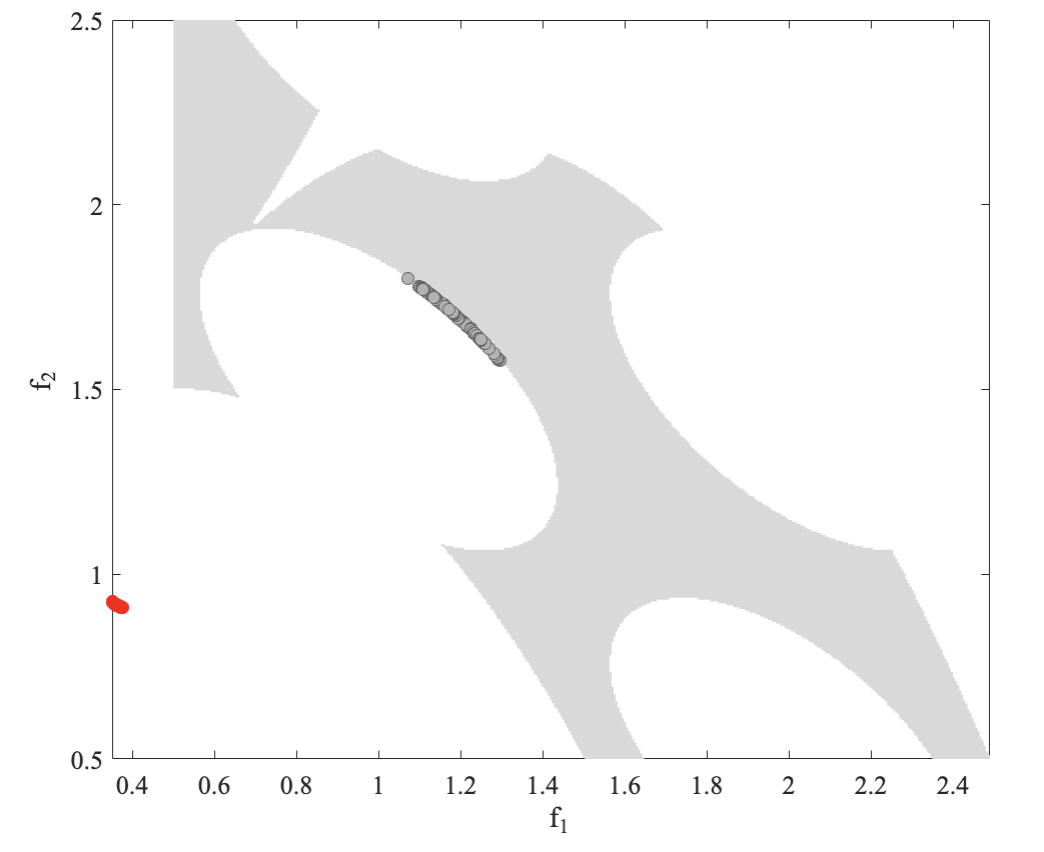
\includegraphics[width=0.7\linewidth]{fig/dascomp1}
  \caption{EMCMO on DASCOMP1 after 10000 function evaluations}
  \label{fig:dascomp1}
\end{figure}




\subsection{Algorithm}
\label{sec:algorithm}
\subsubsection{Framework}
This algorithm use three coevoled populations to solve the CMOPs.

At first, three populations is initialized, each of them has its own goal. The first one is the main population, which is used to approximate the constraint Pareto front. Both the second and the third population are auxiliary populations ignoring the constraints, while they each have different goals. The algorithm of mating, mutation enviroment selection for it is mainly based on the SPEA2 and CDP.

The main function of the second population is to converge to the unconstrained Pareto front, it works as a pioneer to explore the search space and lead the other two populations towars the pareto front. It also utilize SPEA2 as the backbone.

The third population is used to maintain the diversity of the solutions, it works as a exploration team to focus on the rare, novel and useful solutions to introduction new directions helping thee other two populations to escape from local optima and to cover more of whole Pareto front. Notably, this population directly use the algorithm called {\bf MOEA/D-M2M}\cite[m2m]{m2m}, which is a multi-objective evolutionary algorithm based on decomposition. The reason why it's chosen is that it's a very simple algorithm and it's very effective in maintaining the diversity of the solutions. It divde the objectives into several subproblems and optimize them separately, which is very similar to {\bf MOEA/D}\cite{moead}. But it's different from MOEA/D in that it didn't try to some decomposition and aggregation methods to convert the multi-objective problem into a single-objective problem, instead it just divide evenly the objective space into several subspaces and optimize them separately using dominance relation.

This way it can maintain the diversity of the solutions very well, but it's not very effective in convergence. So it's just used to aid the other two populations.




\subsubsection{Size Adjustment}
One of the difficulties of three population approach is that more computation resource is required. So to alleviate this problem, a dynamic methods is design to adjust the relative size between the second and the third population. A running average of successful rate of each auxiliary population is recorded and used to achieve.

\begin{algorithm}
  \SetAlgoLined
  \DontPrintSemicolon
  \KwIn{$N$ (population size), $\bar{N}$ (archive size), $T$ (maximum number of generations)}
  \KwOut{$A$ (nondominated set)}
  \BlankLine
  \tcp{SPEA2 Main Loop}
  Initialization: Generate an initial population $P_0$ and create the empty archive (external set) $P_0 = \emptyset$. Set $t = 0$.\;
  Fitness assignment: Calculate fitness values of individuals in $P_t$ and $P_t$ (cf. Section 3.1).\;
  Environmental selection: Copy all nondominated individuals in $P_t$ and $P_t$ to $P_{t+1}$. If size of $P_{t+1}$ exceeds $N$ then reduce $P_{t+1}$ by means of the truncation operator, otherwise if size of $P_{t+1}$ is less than $N$ then fill $P_{t+1}$ with dominated individuals in $P_t$ and $P_t$ (cf. Section 3.2).\;
  Termination: If $t \geq T$ or another stopping criterion is satisfied then set $A$ to the set of decision vectors represented by the nondominated individuals in $P_{t+1}$. Stop.\;
  Mating selection: Perform binary tournament selection with replacement on $P_{t+1}$ in order to fill the mating pool.\;
  \caption{SPEA2 Main Loop}
\end{algorithm}

% \begin{algorithm}
%   \SetAlgoLined
%   \DontPrintSemicolon
%   \KwIn{$N$ (population size, 种群大小), $\bar{N}$ (archive size, 归档大小), $T$ (maximum number of generations, 最大代数)}
%   \KwOut{$A$ (nondominated set, 非支配集)}
%   \BlankLine
%   \tcp{SPEA2主循环}
%   Initialization (初始化): 生成初始种群 $P_0$ 并创建空归档(外部集)$\bar{P_0} = \emptyset$。设置 $t = 0$。\;
%   \Begin{
%     \While{true}{
%       Fitness assignment (适应度分配): 计算 $P_t$ 和 $\bar{P_t}$ 中个体的适应度值。\;
%       Environmental selection (环境选择): 将 $P_t$ 和 $\bar{P_t}$ 中所有非支配个体复制到 $\bar{P_{t+1}}$。如果 $\bar{P_{t+1}}$ 的大小超过 $\bar{N}$,则通过截断操作减少 $\bar{P_{t+1}}$ 的大小,否则如果 $\bar{P_{t+1}}$ 的大小小于 $\bar{N}$,则用 $P_t$ 和 $\bar{P_t}$ 中的支配个体填充 $\bar{P_{t+1}}$\;
%       Mating selection (交配选择): 对 $\bar{P_{t+1}}$ 进行二元锦标赛选择以填充交配池。\;
%       Recombination and Mutation(交叉变异): 利用交配池中的个体应用交叉和变异算子, 将得到的种群设置为$P_{t+1}$\;
%       Update $t$.\;
%       Termination (是否终止): 如果 $t \geq T$ 或满足其他停止条件,则将 $A$ 设置为 $\bar{P_{t+1}}$ 中非支配个体所代表的决策向量集合。停止。\;
%     }
%   }
%   \caption{SPEA2主循环}
% \end{algorithm}


% \begin{algorithm}
%   \SetAlgoLined
%   \KwResult{Find a set of Pareto-optimal solutions (找到一组帕累托最优解)}
%   initialization (初始化)\;
%   \While{termination condition not met (未达到终止条件)}{
%     fitness assignment (适应度分配)\;
%     environmental selection (环境选择)\;
%     mating selection (交配选择)\;
%     crossover and mutation (交叉和变异)\;
%   }
%   \caption{Strength Pareto Evolutionary Algorithm 2 (SPEA2)}
% \end{algorithm}


% \begin{algorithm}
%   \SetAlgoLined
%   \DontPrintSemicolon
%   \KwResult{Best solution found by the genetic algorithm}
%   \KwIn{Fitness function $f$, population size $N$, crossover rate $p_c$, mutation rate $p_m$}
%   \Begin{
%     population $\leftarrow$ initializePopulation($N$)\;
%     \ForEach{individual in population}{
%       evaluateFitness(individual, $f$)\;
%     }
%     \While{termination condition not met}{
%       parents $\leftarrow$ selectParents(population)\;
%       offspring $\leftarrow$ crossover(parents, $p_c$)\;
%       mutate(offspring, $p_m$)\;
%       \ForEach{child in offspring}{
%         evaluateFitness(child, $f$)\;
%       }
%       population $\leftarrow$ selectNextGeneration(population, offspring)\;
%     }
%     \KwRet{getBestIndividual(population)}
%   }
%   \caption{Pseudocode for a Genetic Algorithm}
% \end{algorithm}

% \begin{algorithm}
%   \DontPrintSemicolon
%   \SetAlgoLined
%   \SetKwInput{KwData}{Input}
%   \SetKwInput{KwResult}{Output}
%   \KwData{Population $P$}
%   \KwResult{A set of non-dominated fronts $F$}
%   \BlankLine
%   \SetKwFunction{FMain}{fastNonDominatedSort}
%   \SetKwProg{Fn}{Function}{:}{}
%   \Fn{\FMain{$P$}}{
%     $F_1 \leftarrow \varnothing$\;
%     \ForEach{$p \in P$}{
%       $S_p \leftarrow \varnothing$\;
%       $n_p \leftarrow 0$\;
%       \ForEach{$q \in P$}{
%         \uIf{$p$ dominates $q$}{
%           $S_p \leftarrow S_p \cup \{q\}$\;
%         }
%         \ElseIf{$q$ dominates $p$}{
%           $n_p \leftarrow n_p + 1$\;
%         }
%       }
%       \If{$n_p == 0$}{
%         $p.rank \leftarrow 1$\;
%         $F_1 \leftarrow F_1 \cup \{p\}$\;
%       }
%     }
%     $i \leftarrow 1$\;
%     \While{$F_i \neq \varnothing$}{
%       $Q \leftarrow \varnothing$\;
%       \ForEach{$p \in F_i$}{
%         \ForEach{$q \in S_p$}{
%           $n_q \leftarrow n_q - 1$\;
%           \If{$n_q == 0$}{
%             $q.rank \leftarrow i+1$\;
%             $Q \leftarrow Q \cup \{q\}$\;
%           }
%         }
%       }
%       $i \leftarrow i + 1$\;
%       $F_i \leftarrow Q$\;
%     }
%     \Return{$F$}\;
%   }
%   \caption{Fast Non-Dominated Sort}
% \end{algorithm}

% \begin{algorithm}
%   \DontPrintSemicolon
%   \SetAlgoLined
%   \SetKwInput{KwData}{Input}
%   \SetKwInput{KwResult}{Output}
%   \KwData{Non-dominated front $F$}
%   \KwResult{Crowding distance assignment for each individual in $F$}
%   \BlankLine
%   \SetKwFunction{FCrowding}{crowdingDistanceAssignment}
%   \SetKwProg{Fn}{Function}{:}{}
%   \Fn{\FCrowding{$F$}}{
%     $l \leftarrow$ size of $F$\;
%     \ForEach{individual $i \in F$}{
%       $i.distance \leftarrow 0$\;
%     }
%     \For{$m \leftarrow 1$ \KwTo number of objectives}{
%       $F \leftarrow$ sort($F$, $m$)\; \tcp{根据第$m$个目标进行排序}
%       $F[1].distance \leftarrow F[l].distance \leftarrow \infty$\; \tcp{边界点拥挤距离设为无穷大}
%       \For{$i \leftarrow 2$ \KwTo $l-1$}{
%         $F[i].distance \leftarrow F[i].distance + \frac{F[i+1].m - F[i-1].m}{F[l].m - F[1].m}$\;
%       }
%     }
%     \Return{$F$}\;
%   }
%   \caption{Crowding Distance Assignment in NSGA-II}
% \end{algorithm}


\begin{algorithm}
  \DontPrintSemicolon
  \SetAlgoLined
  \KwIn{population $P(\tau)$, the tournament size $t \in \{1,2,\ldots,N\}$}
  \KwOut{The population after selection $P(\tau)'$}

  \SetKwFunction{FTournament}{tournament}
  \SetKwProg{Fn}{Function}{:}{}
  \Fn{\FTournament{$t, J_1, \ldots, J_N$}}{
    \For{$i \leftarrow 1$ \KwTo $N$}{
      $J_i' \leftarrow$ best fit individual out of $t$ randomly picked individuals from $\{J_1, \ldots, J_N\}$\;

    }
  }
  \Return{$\{J_1', \ldots, J_N'\}$}\;
  \caption{Tournament Selection}
\end{algorithm}


\begin{algorithm}
  \SetAlgoLined
  \DontPrintSemicolon
  \KwResult{遗传算法找到的最佳解}
  \KwIn{适应度函数 $f$, 种群大小 $N$, 交叉率 $p_c$, 变异率 $p_m$}
  \Begin{
    种群 $\leftarrow$ 初始化种群($N$)\;
    \ForEach{个体 in 种群}{
      计算适应度(个体, $f$)\;
    }
    \While{未达到终止条件}{
      父代 $\leftarrow$ 选择父代(种群)\;
      子代 $\leftarrow$ 交叉(父代, $p_c$)\;
      变异(子代, $p_m$)\;
      \ForEach{孩子 in 子代}{
        计算适应度(孩子, $f$)\;
      }
      种群 $\leftarrow$ 选择下一代种群(种群, 子代)\;
    }
    \KwRet{获得最佳个体(种群)}
  }
  \caption{遗传算法的伪代码}
\end{algorithm}

\subsubsection{Duplication Remoal}
Beacuse of the inter-transfer of knowledge between three population

\subsubsection*{Transfer Scheme}

\subsubsection{Stop Criterion}

\subsubsection{Stage Analysis}





\subsection{Template Parameters}

In addition to specifying the {\itshape template style} to be used in
formatting your work, there are a number of {\itshape template parameters}
which modify some part of the applied template style. A complete list
of these parameters can be found in the {\itshape \LaTeX\ User's Guide.}

Frequently-used parameters, or combinations of parameters, include:
\begin{itemize}
  \item {\verb|anonymous,review|}: Suitable for a ``double-blind''
        conference submission. Anonymizes the work and includes line
        numbers. Use with the \verb|\acmSubmissionID| command to print the
        submission's unique ID on each page of the work.
  \item{\verb|authorversion|}: Produces a version of the work suitable
        for posting by the author.
  \item{\verb|screen|}: Produces colored hyperlinks.
\end{itemize}

This document uses the following string as the first command in the
source file:
\begin{verbatim}
\documentclass[sigconf]{acmart}
\end{verbatim}

\section{Modifications}

Modifying the template --- including but not limited to: adjusting
margins, typeface sizes, line spacing, paragraph and list definitions,
and the use of the \verb|\vspace| command to manually adjust the
vertical spacing between elements of your work --- is not allowed.

  {\bfseries Your document will be returned to you for revision if
    modifications are discovered.}

\section{Typefaces}

The ``\verb|acmart|'' document class requires the use of the
``Libertine'' typeface family. Your \TeX\ installation should include
this set of packages. Please do not substitute other typefaces. The
``\verb|lmodern|'' and ``\verb|ltimes|'' packages should not be used,
as they will override the built-in typeface families.

\section{Title Information}

The title of your work should use capital letters appropriately -
\url{https://capitalizemytitle.com/} has useful rules for
capitalization. Use the {\verb|title|} command to define the title of
your work. If your work has a subtitle, define it with the
  {\verb|subtitle|} command.  Do not insert line breaks in your title.

If your title is lengthy, you must define a short version to be used
in the page headers, to prevent overlapping text. The \verb|title|
command has a ``short title'' parameter:
\begin{verbatim}
  \title[short title]{full title}
\end{verbatim}

\section{Authors and Affiliations}

Each author must be defined separately for accurate metadata
identification. Multiple authors may share one affiliation. Authors'
names should not be abbreviated; use full first names wherever
possible. Include authors' e-mail addresses whenever possible.

Grouping authors' names or e-mail addresses, or providing an ``e-mail
alias,'' as shown below, is not acceptable:
\begin{verbatim}
  \author{Brooke Aster, David Mehldau}
  \email{dave,judy,steve@university.edu}
  \email{firstname.lastname@phillips.org}
\end{verbatim}

The \verb|authornote| and \verb|authornotemark| commands allow a note
to apply to multiple authors --- for example, if the first two authors
of an article contributed equally to the work.

If your author list is lengthy, you must define a shortened version of
the list of authors to be used in the page headers, to prevent
overlapping text. The following command should be placed just after
the last \verb|\author{}| definition:
\begin{verbatim}
  \renewcommand{\shortauthors}{McCartney, et al.}
\end{verbatim}
Omitting this command will force the use of a concatenated list of all
of the authors' names, which may result in overlapping text in the
page headers.

The article template's documentation, available at
\url{https://www.acm.org/publications/proceedings-template}, has a
complete explanation of these commands and tips for their effective
use.

Note that authors' addresses are mandatory for journal articles.

\section{Rights Information}

Authors of any work published by ACM will need to complete a rights
form. Depending on the kind of work, and the rights management choice
made by the author, this may be copyright transfer, permission,
license, or an OA (open access) agreement.

Regardless of the rights management choice, the author will receive a
copy of the completed rights form once it has been submitted. This
form contains \LaTeX\ commands that must be copied into the source
document. When the document source is compiled, these commands and
their parameters add formatted text to several areas of the final
document:
\begin{itemize}
  \item the ``ACM Reference Format'' text on the first page.
  \item the ``rights management'' text on the first page.
  \item the conference information in the page header(s).
\end{itemize}

Rights information is unique to the work; if you are preparing several
works for an event, make sure to use the correct set of commands with
each of the works.

The ACM Reference Format text is required for all articles over one
page in length, and is optional for one-page articles (abstracts).

\section{CCS Concepts and User-Defined Keywords}

Two elements of the ``acmart'' document class provide powerful
taxonomic tools for you to help readers find your work in an online
search.

The ACM Computing Classification System ---
\url{https://www.acm.org/publications/class-2012} --- is a set of
classifiers and concepts that describe the computing
discipline. Authors can select entries from this classification
system, via \url{https://dl.acm.org/ccs/ccs.cfm}, and generate the
commands to be included in the \LaTeX\ source.

User-defined keywords are a comma-separated list of words and phrases
of the authors' choosing, providing a more flexible way of describing
the research being presented.

CCS concepts and user-defined keywords are required for for all
articles over two pages in length, and are optional for one- and
two-page articles (or abstracts).

\section{Sectioning Commands}

Your work should use standard \LaTeX\ sectioning commands:
\verb|section|, \verb|subsection|, \verb|subsubsection|, and
\verb|paragraph|. They should be numbered; do not remove the numbering
from the commands.

Simulating a sectioning command by setting the first word or words of
a paragraph in boldface or italicized text is {\bfseries not allowed.}

\section{Tables}

The ``\verb|acmart|'' document class includes the ``\verb|booktabs|''
package --- \url{https://ctan.org/pkg/booktabs} --- for preparing
high-quality tables.

Table captions are placed {\itshape above} the table.

Because tables cannot be split across pages, the best placement for
them is typically the top of the page nearest their initial cite.  To
ensure this proper ``floating'' placement of tables, use the
environment \textbf{table} to enclose the table's contents and the
table caption.  The contents of the table itself must go in the
\textbf{tabular} environment, to be aligned properly in rows and
columns, with the desired horizontal and vertical rules.  Again,
detailed instructions on \textbf{tabular} material are found in the
\textit{\LaTeX\ User's Guide}.

Immediately following this sentence is the point at which
Table~\ref{tab:freq} is included in the input file; compare the
placement of the table here with the table in the printed output of
this document.

\begin{table}
  \caption{Frequency of Special Characters}
  \label{tab:freq}
  \begin{tabular}{ccl}
    \toprule
    Non-English or Math & Frequency   & Comments          \\
    \midrule
    \O                  & 1 in 1,000  & For Swedish names \\
    $\pi$               & 1 in 5      & Common in math    \\
    \$                  & 4 in 5      & Used in business  \\
    $\Psi^2_1$          & 1 in 40,000 & Unexplained usage \\
    \bottomrule
  \end{tabular}
\end{table}

To set a wider table, which takes up the whole width of the page's
live area, use the environment \textbf{table*} to enclose the table's
contents and the table caption.  As with a single-column table, this
wide table will ``float'' to a location deemed more
desirable. Immediately following this sentence is the point at which
Table~\ref{tab:commands} is included in the input file; again, it is
instructive to compare the placement of the table here with the table
in the printed output of this document.

\begin{table*}
  \caption{Some Typical Commands}
  \label{tab:commands}
  \begin{tabular}{ccl}
    \toprule
    Command                    & A Number & Comments         \\
    \midrule
    \texttt{{\char'134}author} & 100      & Author           \\
    \texttt{{\char'134}table}  & 300      & For tables       \\
    \texttt{{\char'134}table*} & 400      & For wider tables \\
    \bottomrule
  \end{tabular}
\end{table*}

Always use midrule to separate table header rows from data rows, and
use it only for this purpose. This enables assistive technologies to
recognise table headers and support their users in navigating tables
more easily.

\section{Math Equations}
You may want to display math equations in three distinct styles:
inline, numbered or non-numbered display.  Each of the three are
discussed in the next sections.

\subsection{Inline (In-text) Equations}
A formula that appears in the running text is called an inline or
in-text formula.  It is produced by the \textbf{math} environment,
which can be invoked with the usual
\texttt{{\char'134}begin\,\ldots{\char'134}end} construction or with
the short form \texttt{\$\,\ldots\$}. You can use any of the symbols
and structures, from $\alpha$ to $\omega$, available in
\LaTeX~\cite{Lamport:LaTeX}; this section will simply show a few
examples of in-text equations in context. Notice how this equation:
\begin{math}
  \lim_{n\rightarrow \infty}x=0
\end{math},
set here in in-line math style, looks slightly different when
set in display style.  (See next section).

\subsection{Display Equations}
A numbered display equation---one set off by vertical space from the
text and centered horizontally---is produced by the \textbf{equation}
environment. An unnumbered display equation is produced by the
\textbf{displaymath} environment.

Again, in either environment, you can use any of the symbols and
structures available in \LaTeX\@; this section will just give a couple
of examples of display equations in context.  First, consider the
equation, shown as an inline equation above:
\begin{equation}
  \lim_{n\rightarrow \infty}x=0
\end{equation}
Notice how it is formatted somewhat differently in
the \textbf{displaymath}
environment.  Now, we'll enter an unnumbered equation:
\begin{displaymath}
  \sum_{i=0}^{\infty} x + 1
\end{displaymath}
and follow it with another numbered equation:
\begin{equation}
  \sum_{i=0}^{\infty}x_i=\int_{0}^{\pi+2} f
\end{equation}
just to demonstrate \LaTeX's able handling of numbering.

\section{Figures}

The ``\verb|figure|'' environment should be used for figures. One or
more images can be placed within a figure. If your figure contains
third-party material, you must clearly identify it as such, as shown
in the example below.
\begin{figure}[h]
  \centering
  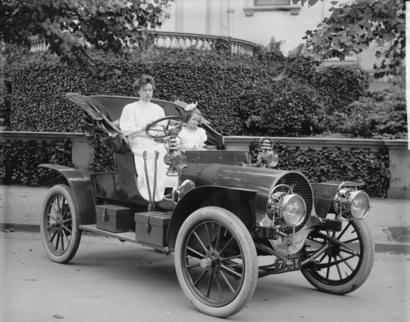
\includegraphics[width=\linewidth]{sample-franklin}
  \caption{1907 Franklin Model D roadster. Photograph by Harris \&
    Ewing, Inc. [Public domain], via Wikimedia
    Commons. (\url{https://goo.gl/VLCRBB}).}
  \Description{A woman and a girl in white dresses sit in an open car.}
\end{figure}

Your figures should contain a caption which describes the figure to
the reader.

Figure captions are placed {\itshape below} the figure.

Every figure should also have a figure description unless it is purely
decorative. These descriptions convey what’s in the image to someone
who cannot see it. They are also used by search engine crawlers for
indexing images, and when images cannot be loaded.

A figure description must be unformatted plain text less than 2000
characters long (including spaces).  {\bfseries Figure descriptions
    should not repeat the figure caption – their purpose is to capture
    important information that is not already provided in the caption or
    the main text of the paper.} For figures that convey important and
complex new information, a short text description may not be
adequate. More complex alternative descriptions can be placed in an
appendix and referenced in a short figure description. For example,
provide a data table capturing the information in a bar chart, or a
structured list representing a graph.  For additional information
regarding how best to write figure descriptions and why doing this is
so important, please see
\url{https://www.acm.org/publications/taps/describing-figures/}.

\subsection{The ``Teaser Figure''}

A ``teaser figure'' is an image, or set of images in one figure, that
are placed after all author and affiliation information, and before
the body of the article, spanning the page. If you wish to have such a
figure in your article, place the command immediately before the
\verb|\maketitle| command:
\begin{verbatim}
  \begin{teaserfigure}
    \includegraphics[width=\textwidth]{sampleteaser}
    \caption{figure caption}
    \Description{figure description}
  \end{teaserfigure}
\end{verbatim}

\section{Citations and Bibliographies}

The use of \BibTeX\ for the preparation and formatting of one's
references is strongly recommended. Authors' names should be complete
--- use full first names (``Donald E. Knuth'') not initials
(``D. E. Knuth'') --- and the salient identifying features of a
reference should be included: title, year, volume, number, pages,
article DOI, etc.

The bibliography is included in your source document with these two
commands, placed just before the \verb|\end{document}| command:
\begin{verbatim}
  \bibliographystyle{ACM-Reference-Format}
  \bibliography{bibfile}
\end{verbatim}
where ``\verb|bibfile|'' is the name, without the ``\verb|.bib|''
suffix, of the \BibTeX\ file.

Citations and references are numbered by default. A small number of
ACM publications have citations and references formatted in the
``author year'' style; for these exceptions, please include this
command in the {\bfseries preamble} (before the command
``\verb|\begin{document}|'') of your \LaTeX\ source:
\begin{verbatim}
  \citestyle{acmauthoryear}
\end{verbatim}

Some examples.  A paginated journal article \cite{Abril07}, an
enumerated journal article \cite{Cohen07}, a reference to an entire
issue \cite{JCohen96}, a monograph (whole book) \cite{Kosiur01}, a
monograph/whole book in a series (see 2a in spec. document)
\cite{Harel79}, a divisible-book such as an anthology or compilation
\cite{Editor00} followed by the same example, however we only output
the series if the volume number is given \cite{Editor00a} (so
Editor00a's series should NOT be present since it has no vol. no.),
a chapter in a divisible book \cite{Spector90}, a chapter in a
divisible book in a series \cite{Douglass98}, a multi-volume work as
book \cite{Knuth97}, a couple of articles in a proceedings (of a
conference, symposium, workshop for example) (paginated proceedings
article) \cite{Andler79, Hagerup1993}, a proceedings article with
all possible elements \cite{Smith10}, an example of an enumerated
proceedings article \cite{VanGundy07}, an informally published work
\cite{Harel78}, a couple of preprints \cite{Bornmann2019,
  AnzarootPBM14}, a doctoral dissertation \cite{Clarkson85}, a
master's thesis: \cite{anisi03}, an online document / world wide web
resource \cite{Thornburg01, Ablamowicz07, Poker06}, a video game
(Case 1) \cite{Obama08} and (Case 2) \cite{Novak03} and \cite{Lee05}
and (Case 3) a patent \cite{JoeScientist001}, work accepted for
publication \cite{rous08}, 'YYYYb'-test for prolific author
\cite{SaeediMEJ10} and \cite{SaeediJETC10}. Other cites might
contain 'duplicate' DOI and URLs (some SIAM articles)
\cite{Kirschmer:2010:AEI:1958016.1958018}. Boris / Barbara Beeton:
multi-volume works as books \cite{MR781536} and \cite{MR781537}. A
couple of citations with DOIs:
\cite{2004:ITE:1009386.1010128,Kirschmer:2010:AEI:1958016.1958018}. Online
citations: \cite{TUGInstmem, Thornburg01, CTANacmart}. Artifacts:
\cite{R} and \cite{UMassCitations}.

\section{Acknowledgments}

Identification of funding sources and other support, and thanks to
individuals and groups that assisted in the research and the
preparation of the work should be included in an acknowledgment
section, which is placed just before the reference section in your
document.

This section has a special environment:
\begin{verbatim}
  \begin{acks}
  ...
  \end{acks}
\end{verbatim}
so that the information contained therein can be more easily collected
during the article metadata extraction phase, and to ensure
consistency in the spelling of the section heading.

Authors should not prepare this section as a numbered or unnumbered {\verb|\section|}; please use the ``{\verb|acks|}'' environment.

\section{Appendices}

If your work needs an appendix, add it before the
``\verb|\end{document}|'' command at the conclusion of your source
document.

Start the appendix with the ``\verb|appendix|'' command:
\begin{verbatim}
  \appendix
\end{verbatim}
and note that in the appendix, sections are lettered, not
numbered. This document has two appendices, demonstrating the section
and subsection identification method.

\section{SIGCHI Extended Abstracts}

The ``\verb|sigchi-a|'' template style (available only in \LaTeX\ and
not in Word) produces a landscape-orientation formatted article, with
a wide left margin. Three environments are available for use with the
``\verb|sigchi-a|'' template style, and produce formatted output in
the margin:
\begin{itemize}
  \item {\verb|sidebar|}:  Place formatted text in the margin.
  \item {\verb|marginfigure|}: Place a figure in the margin.
  \item {\verb|margintable|}: Place a table in the margin.
\end{itemize}

%%
%% The acknowledgments section is defined using the "acks" environment
%% (and NOT an unnumbered section). This ensures the proper
%% identification of the section in the article metadata, and the
%% consistent spelling of the heading.
\begin{acks}
  To Robert, for the bagels and explaining CMYK and color spaces.
\end{acks}

%%
%% The next two lines define the bibliography style to be used, and
%% the bibliography file.
\bibliographystyle{ACM-Reference-Format}
\bibliography{sample-base}

%%
%% If your work has an appendix, this is the place to put it.
\appendix

\section{Research Methods}

\subsection{Part One}

Lorem ipsum dolor sit amet, consectetur adipiscing elit. Morbi
malesuada, quam in pulvinar varius, metus nunc fermentum urna, id
sollicitudin purus odio sit amet enim. Aliquam ullamcorper eu ipsum
vel mollis. Curabitur quis dictum nisl. Phasellus vel semper risus, et
lacinia dolor. Integer ultricies commodo sem nec semper.

\subsection{Part Two}

Etiam commodo feugiat nisl pulvinar pellentesque. Etiam auctor sodales
ligula, non varius nibh pulvinar semper. Suspendisse nec lectus non
ipsum convallis congue hendrerit vitae sapien. Donec at laoreet
eros. Vivamus non purus placerat, scelerisque diam eu, cursus
ante. Etiam aliquam tortor auctor efficitur mattis.

\section{Online Resources}

Nam id fermentum dui. Suspendisse sagittis tortor a nulla mollis, in
pulvinar ex pretium. Sed interdum orci quis metus euismod, et sagittis
enim maximus. Vestibulum gravida massa ut felis suscipit
congue. Quisque mattis elit a risus ultrices commodo venenatis eget
dui. Etiam sagittis eleifend elementum.

Nam interdum magna at lectus dignissim, ac dignissim lorem
rhoncus. Maecenas eu arcu ac neque placerat aliquam. Nunc pulvinar
massa et mattis lacinia.

\end{document}
\endinput
%%
%% End of file `sample-sigconf.tex'.
